% LaTeX path to the root directory of the current project, from the directory in which this file resides
% and path to econtexPaths which defines the rest of the paths like \FigDir
\providecommand{\econtexRoot}{}\renewcommand{\econtexRoot}{.}
\providecommand{\econtexPaths}{}\renewcommand{\econtexPaths}{\econtexRoot/Resources/econtexPaths}
% The \commands below are required to allow sharing of the same base code via Github between TeXLive on a local machine and Overleaf (which is a proxy for "a standard distribution of LaTeX").  This is an ugly solution to the requirement that custom LaTeX packages be accessible, and that Overleaf prohibits symbolic links
\providecommand{\econtex}{\econtexRoot/Resources/texmf-local/tex/latex/econtex}
\providecommand{\econtexSetup}{\econtexRoot/Resources/texmf-local/tex/latex/econtexSetup}
\providecommand{\econtexShortcuts}{\econtexRoot/Resources/texmf-local/tex/latex/econtexShortcuts}
\providecommand{\econtexBibMake}{\econtexRoot/Resources/texmf-local/tex/latex/econtexBibMake}
\providecommand{\econtexBibStyle}{\econtexRoot/Resources/texmf-local/bibtex/bst/econtex}
\providecommand{\econtexBib}{economics}
\providecommand{\notes}{\econtexRoot/Resources/texmf-local/tex/latex/handout}
\providecommand{\handoutSetup}{\econtexRoot/Resources/texmf-local/tex/latex/handoutSetup}
\providecommand{\handoutShortcuts}{\econtexRoot/Resources/texmf-local/tex/latex/handoutShortcuts}
\providecommand{\handoutBibMake}{\econtexRoot/Resources/texmf-local/tex/latex/handoutBibMake}
\providecommand{\handoutBibStyle}{\econtexRoot/Resources/texmf-local/bibtex/bst/handout}

\providecommand{\FigDir}{\econtexRoot/Figures}
\providecommand{\CodeDir}{\econtexRoot/Code}
\providecommand{\DataDir}{\econtexRoot/Data}
\providecommand{\SlideDir}{\econtexRoot/Slides}
\providecommand{\TableDir}{\econtexRoot/Tables}
\providecommand{\ApndxDir}{\econtexRoot/Appendices}

\providecommand{\ResourcesDir}{\econtexRoot/Resources}
\providecommand{\rootFromOut}{..} % Path back to root directory from output-directory
\providecommand{\LaTeXGenerated}{\econtexRoot/LaTeX} % Put generated files in subdirectory
\providecommand{\econtexPaths}{\econtexRoot/Resources/econtexPaths}
\providecommand{\LaTeXInputs}{\econtexRoot/Resources/LaTeXInputs}
\providecommand{\LtxDir}{LaTeX/}
\providecommand{\EqDir}{Equations} % Put generated files in subdirectory

\documentclass[\econtexRoot/ProjectUYA]{subfiles}
% LaTeX path to the root directory of the current project, from the directory in which this file resides
% and path to econtexPaths which defines the rest of the paths like \FigDir
\providecommand{\econtexRoot}{}\renewcommand{\econtexRoot}{.}
\providecommand{\econtexPaths}{}\renewcommand{\econtexPaths}{\econtexRoot/Resources/econtexPaths}
% The \commands below are required to allow sharing of the same base code via Github between TeXLive on a local machine and Overleaf (which is a proxy for "a standard distribution of LaTeX").  This is an ugly solution to the requirement that custom LaTeX packages be accessible, and that Overleaf prohibits symbolic links
\providecommand{\econtex}{\econtexRoot/Resources/texmf-local/tex/latex/econtex}
\providecommand{\econtexSetup}{\econtexRoot/Resources/texmf-local/tex/latex/econtexSetup}
\providecommand{\econtexShortcuts}{\econtexRoot/Resources/texmf-local/tex/latex/econtexShortcuts}
\providecommand{\econtexBibMake}{\econtexRoot/Resources/texmf-local/tex/latex/econtexBibMake}
\providecommand{\econtexBibStyle}{\econtexRoot/Resources/texmf-local/bibtex/bst/econtex}
\providecommand{\econtexBib}{economics}
\providecommand{\notes}{\econtexRoot/Resources/texmf-local/tex/latex/handout}
\providecommand{\handoutSetup}{\econtexRoot/Resources/texmf-local/tex/latex/handoutSetup}
\providecommand{\handoutShortcuts}{\econtexRoot/Resources/texmf-local/tex/latex/handoutShortcuts}
\providecommand{\handoutBibMake}{\econtexRoot/Resources/texmf-local/tex/latex/handoutBibMake}
\providecommand{\handoutBibStyle}{\econtexRoot/Resources/texmf-local/bibtex/bst/handout}

\providecommand{\FigDir}{\econtexRoot/Figures}
\providecommand{\CodeDir}{\econtexRoot/Code}
\providecommand{\DataDir}{\econtexRoot/Data}
\providecommand{\SlideDir}{\econtexRoot/Slides}
\providecommand{\TableDir}{\econtexRoot/Tables}
\providecommand{\ApndxDir}{\econtexRoot/Appendices}

\providecommand{\ResourcesDir}{\econtexRoot/Resources}
\providecommand{\rootFromOut}{..} % Path back to root directory from output-directory
\providecommand{\LaTeXGenerated}{\econtexRoot/LaTeX} % Put generated files in subdirectory
\providecommand{\econtexPaths}{\econtexRoot/Resources/econtexPaths}
\providecommand{\LaTeXInputs}{\econtexRoot/Resources/LaTeXInputs}
\providecommand{\LtxDir}{LaTeX/}
\providecommand{\EqDir}{Equations} % Put generated files in subdirectory

\onlyinsubfile{% https://tex.stackexchange.com/questions/463699/proper-reference-numbers-with-subfiles
    \csname @ifpackageloaded\endcsname{xr-hyper}{%
      \externaldocument{\econtexRoot/BufferStockTheory}% xr-hyper in use; optional argument for url of main.pdf for hyperlinks
    }{%
      \externaldocument{\econtexRoot/BufferStockTheory}% xr in use
    }%
    \renewcommand\labelprefix{}%
    % Initialize the counters via the labels belonging to the main document:
    \setcounter{equation}{\numexpr\getrefnumber{\labelprefix eq:Dummy}\relax}% eq:Dummy is the last number used for an equation in the main text; start counting up from there
}


\onlyinsubfile{\externaldocument{\LaTeXGenerated/ProjectUYA}}

\begin{document}
\begin{figure}[ht]
  \centerline{
    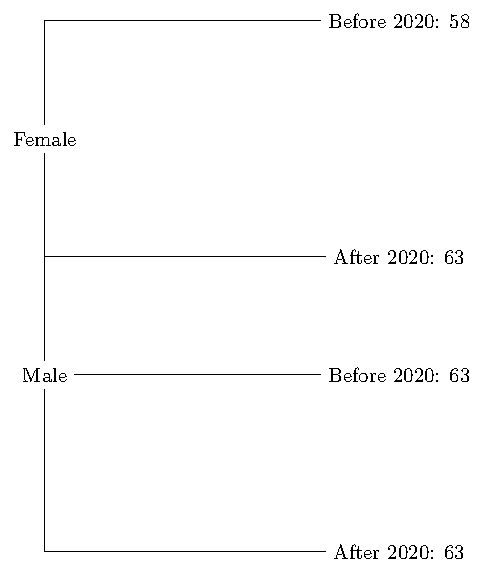
\includegraphics[width=6.0in]{\FigDir/Pension-age}
}
  \caption{Male and Female retirement age} \label{fig:Timeline}

\end{figure}

 % Store the tex for standalone compilation
\begin{figure}[tbp]
\centerline{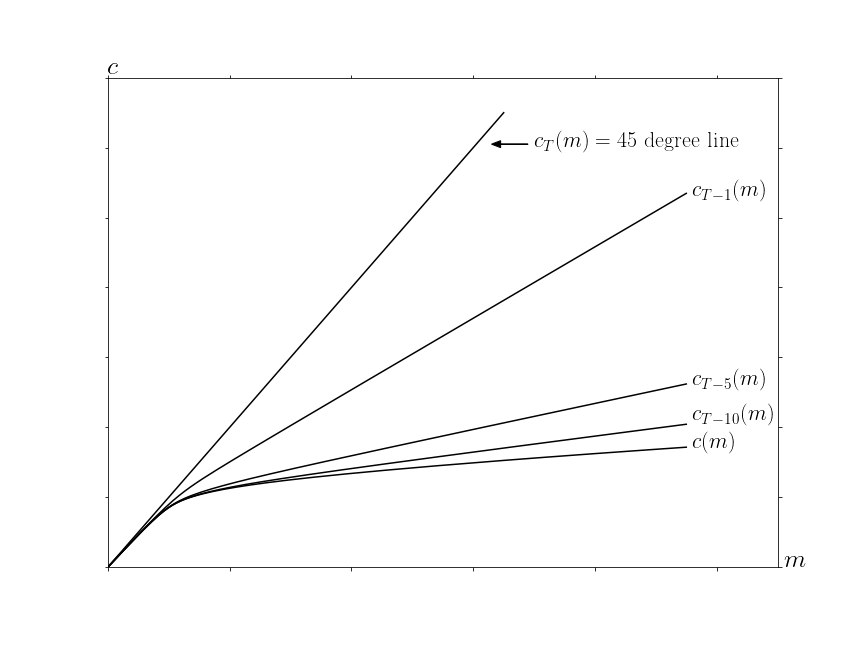
\includegraphics[width=5.25in]{\FigDir/cFuncsConverge}}
\caption{Convergence of the Consumption Rules}
\label{fig:cFuncsConverge}
\end{figure}

        \node (thorn) {$\Pat$};
        \node (gamma) [right of = thorn, xshift = 5cm] {$\PGro$};
        \node (rfree) [below of = thorn]{$\mathsf{\Rfree}$};
        \node (pffvacFac) [right of = rfree] 
        {$\underbrace{\mathsf{\Rfree}^{1/\CRRA}\PGro^{1 - 1/\CRRA}}_{\PFVAF}$};
        \node (pThorn) [left of = thorn] {$\pZero^{1/\rho}\Pat$};
        \node (compgamma) [above of = gamma, xshift = -5cm, yshift = -2.5cm]{$\PGroAdj$};
        \node (fvacFac) [right of = thorn, yshift = -2cm]{$\mathsf{\Rfree}^{1/\CRRA}\PGrouAdj^{1 - 1/\CRRA}$};
        \draw[->] (thorn) to node {${\GICAbs}$} (gamma);
        \draw[->] (thorn) to node [swap] {${\RIC}$} (rfree);
        \draw[->] (thorn) to node [swap] {${\PFFVAC}$} (pffvacFac);
        \draw[->] (gamma) to node {${\FHWC}$} (pffvacFac);
        \draw[->] (pffvacFac) to node {${\FHWC}$} (rfree);
        \draw[->] (pThorn) to node [above]{because $\wp < 1$} (thorn);
        \draw[->] (pThorn) to node [swap] {${\WRIC}$} (rfree);
        \draw[->] (compgamma) to node [rotate=-35,xshift=-2.2cm,yshift=+0.05cm]{because $\underline{\psi} < 1$ and $\uline{\PGro} \equiv \underline{\psi} \PGro$} (gamma);
        \draw[->] (thorn) to node {${\GICNrm}$} (compgamma);
        \draw[->] (fvacFac) to node [rotate=-90,xshift=-1.6cm,yshift=0.25cm]{because $\PGrouAdj < \PGro$} (pffvacFac);
        \draw[->] (thorn) to node {${\FVAC}$} (fvacFac);

\hypertarget{FVACnotGIC}{}
\begin{figure}[tbp]
\centerline{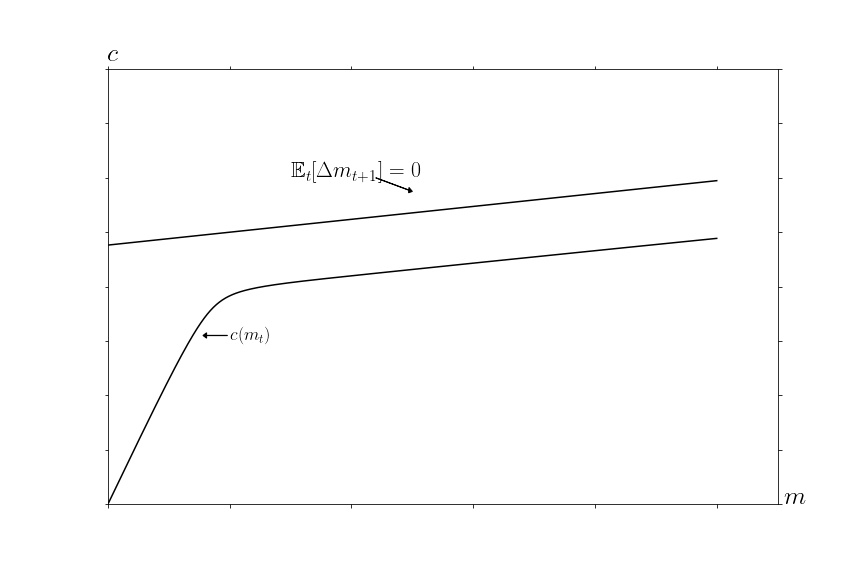
\includegraphics[width=6in]{\FigDir/FVACnotGIC}}
\caption{Example Solution under \{\FVAC,\cncl{\GICNrm}\}}
\label{fig:FVACnotGIC}
\end{figure}

% Could not get fonts to work right for svg version of this figure for web; so use png
\ifthenelse{\boolean{Web}}{
\begin{figure}[tbp]
\centerline{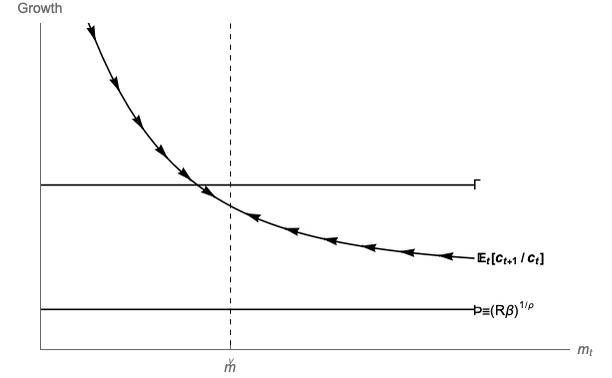
\includegraphics[width=8in]{\FigDir/cGroTargetFig.png}}
\caption{`Stable' $\mRat$ Values and Expected Growth Rates}
\label{fig:cGroTargetFig}
\end{figure}
}{
\begin{figure}[tbp]
\centerline{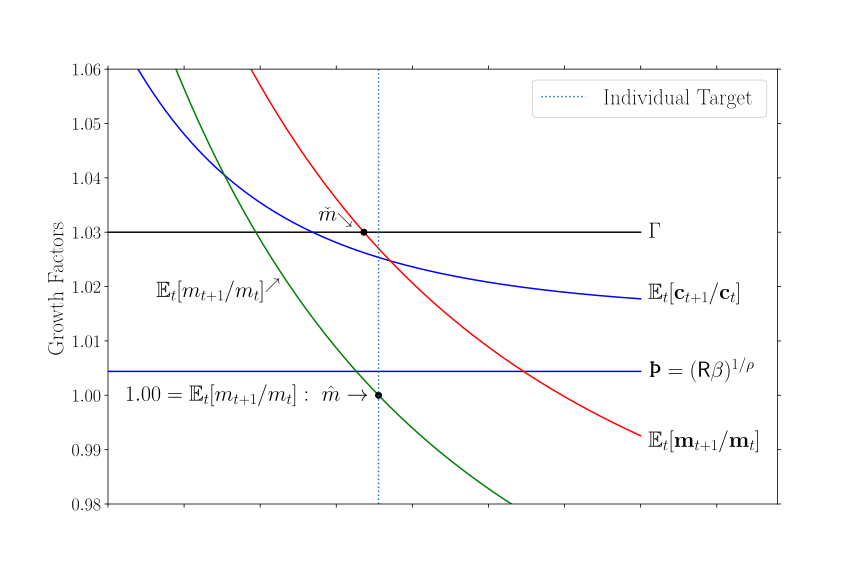
\includegraphics[width=6in]{\FigDir/cGroTargetFig}}
\caption{`Stable' $\mRat$ Values and Expected Growth Factors}
\label{fig:cGroTargetFig}
\end{figure}
}

\hypertarget{MPCLimits}{}
\begin{figure}
\centerline{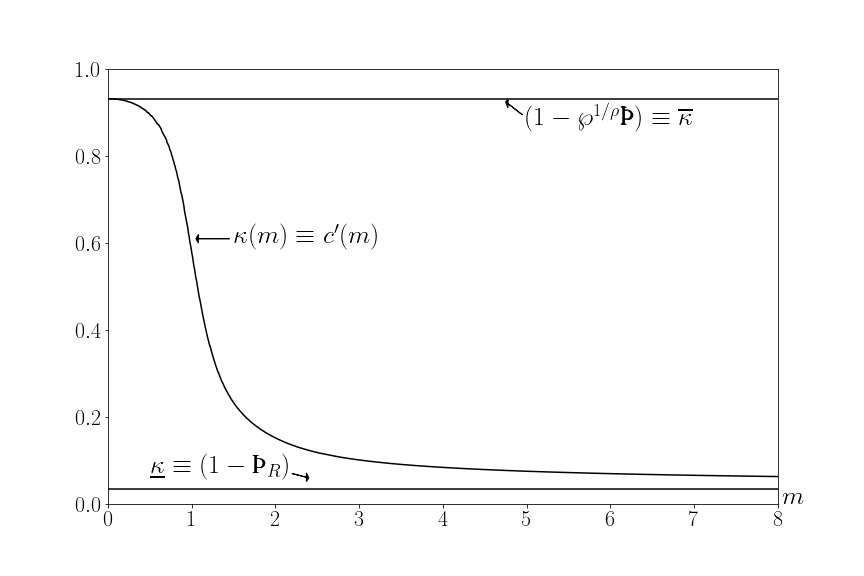
\includegraphics[width=6in]{\FigDir/MPCLimits}}
\caption{Limiting MPC's}
\label{fig:mpclimits}
\end{figure}

\begin{figure}
\centering

\includegraphics[width=6in]{\FigDir/cFuncBounds}
\caption{Upper and Lower Bounds on The Consumption Function}
\label{fig:cFuncBounds}
\end{figure}

\hypertarget{PFGICHoldsFHWCFailsRICFails}{}
\begin{figure}
\centerline{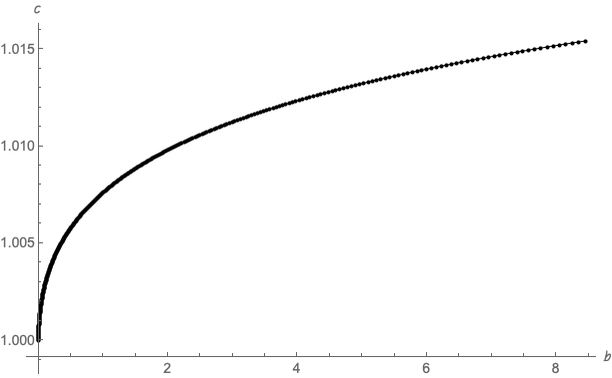
\includegraphics[width=6in]{\FigDir/PFGICHoldsFHWCFailsRICFails}}
\caption{Nondegenerate Consumption Function with $\cncl{\FHWC}$ and \cncl{\RIC}}
\label{fig:PFGICHoldsFHWCFailsRICFails}
\end{figure}



\end{document}
% Local Variables:
% eval: (setq TeX-command-list  (assq-delete-all (car (assoc "BibTeX" TeX-command-list)) TeX-command-list))
% eval: (setq TeX-command-list  (assq-delete-all (car (assoc "BibTeX" TeX-command-list)) TeX-command-list))
% eval: (setq TeX-command-list  (assq-delete-all (car (assoc "BibTeX" TeX-command-list)) TeX-command-list))
% eval: (setq TeX-command-list  (assq-delete-all (car (assoc "BibTeX" TeX-command-list)) TeX-command-list))
% eval: (setq TeX-command-list  (assq-delete-all (car (assoc "Biber"  TeX-command-list)) TeX-command-list))
% eval: (add-to-list 'TeX-command-list '("BibTeX" "bibtex ../LaTeX/%s" TeX-run-BibTeX nil t                                                                              :help "Run BibTeX") t)
% eval: (add-to-list 'TeX-command-list '("BibTeX" "bibtex ../LaTeX/%s" TeX-run-BibTeX nil (plain-tex-mode latex-mode doctex-mode ams-tex-mode texinfo-mode context-mode) :help "Run BibTeX") t)
% tex-bibtex-command: "bibtex ../LaTeX/*"
% TeX-PDF-mode: t
% TeX-file-line-error: t
% TeX-debug-warnings: t
% LaTeX-command-style: (("" "%(PDF)%(latex) %(file-line-error) %(extraopts) -output-directory=../LaTeX %S%(PDFout)"))
% TeX-source-correlate-mode: t
% TeX-parse-self: t
% eval: (cond ((string-equal system-type "darwin") (progn (setq TeX-view-program-list '(("Skim" "/Applications/Skim.app/Contents/SharedSupport/displayline -b %n ../LaTeX/%o %b"))))))
% eval: (cond ((string-equal system-type "gnu/linux") (progn (setq TeX-view-program-list '(("Evince" "evince --page-index=%(outpage) ../LaTeX/%o"))))))
% eval: (cond ((string-equal system-type "gnu/linux") (progn (setq TeX-view-program-selection '((output-pdf "Evince"))))))
% TeX-parse-all-errors: t
% End:
